\documentclass[10pt,journal]{IEEEtran}

\usepackage{amsmath}
\usepackage{siunitx}
\DeclareSIUnit{\torr}{Torr}
\usepackage{graphicx}
\usepackage{subcaption}
\usepackage{cite}
\usepackage{xcolor}
\graphicspath{{images/}}

% ---------------------------------------------------------------------------
% Same \TODO convention used in ASC_Cavity_Paper: renders in red so nothing
% marked here can reach a submitted draft unnoticed.
% ---------------------------------------------------------------------------
\newcommand{\TODO}[1]{\textcolor{red}{\textbf{[TODO: #1]}}}

\begin{document}

\title{RF Characterization of a Sputtered Nb-Coated Copper Cavity at 11\,GHz: Benchmarking Against Bulk Copper and BCS Niobium}

\author{Andre~R.~Juliao,~Andre~Quintero,~Mehrdad~Kiani,~Lance~Cooley,~and~Shreyas~Balachandran%
\thanks{Manuscript submitted for review to the 2026 Applied Superconductivity Conference.}%
\thanks{A.~R.~Juliao and S.~Balachandran are with the Department of Mechanical and Aerospace Engineering, FAMU-FSU College of Engineering, Tallahassee, FL 32310 USA (e-mail: arj14c@fsu.edu).}%
\thanks{A.~Quintero and L.~Cooley are with the National High Magnetic Field Laboratory, Tallahassee, FL 32310 USA.}%
\thanks{M.~Kiani and S.~Balachandran are with the Department of Materials Science and Engineering, FAMU-FSU College of Engineering, Tallahassee, FL 32310 USA.}%
}

\maketitle

\begin{abstract}
\TODO{Write last. Must contain: 2-piece hexagonal Cu/Ta/Nb cavity, 11 GHz, PPMS 2--10 K; $Q_0=1.64\times10^6$, $R_s=213\,\mu\Omega$ at 2 K, $G=350\,\Omega$; $\sim$26$\times$ over measured bare-Cu ($Q_0=62{,}000$), consistent with simulated Cu ceiling ($Q_0=77{,}000$); $\sim$250$\times$ above BCS-Nb $R_s$, attributed to surface roughness not trapped flux; sharp transition at 9.2 K confirms clean film + working Ta barrier. No thesis passage covers this dataset -- draft fresh.}
\end{abstract}

\begin{IEEEkeywords}
Niobium thin films, superconducting cavities, quality factor, surface resistance, BCS theory, axion haloscopes.
\end{IEEEkeywords}

\section{Introduction}

% --- Ported/adapted from thesis Ch.1 "Background and Motivation" (pp.1-2) ---
% Original discusses Nb3Sn broadly; adapted here to motivate the Ta/Nb control
% measurement instead. Your original numbers (Cu Rs~5 m-ohm, Q~3e5; Nb
% Hc2~0.2 T) are kept -- check they still match how you want to frame THIS
% paper's scope before reusing.
Improving cavity quality factor $Q$ is the most accessible route to increasing axion haloscope scan rate, since scan rate scales with $B^4 V^2 Q$ while magnet bore size, field strength, and cost jointly constrain $B$ and $V$~\TODO{cite as in thesis, refs [1] and similar}. Copper has been the primary conductor for high-field RF applications because it can be refined to very high purity (RRR $>$ 300), giving a surface resistance of $\sim$\SI{5}{\milli\ohm} and $Q\sim3\times10^5$ at the frequencies of interest~\cite{ADMX:2009iij}. Superconductors are not limited by the anomalous skin effect that sets this floor for normal metals, and can reach surface resistances orders of magnitude lower~\cite{Ciovati:2014zti}. Conventional superconductors such as niobium, however, have a low upper critical field ($H_{c2}\approx\SI{0.2}{\tesla}$ for Nb) and break down at the fields of interest for axion detection.

% --- Adapted from thesis Ch.1 (Nb3Sn motivation) ---
Nb$_3$Sn represents the most promising near-term solution for high-field superconducting cavities, with $H_{c2}\approx\SI{30}{\tesla}$~\cite{gurevichUseNotUse2011} and compatibility with Cu substrates for superior thermal management~\cite{withanageRapidNbSn2021}. The standard route, vapor diffusion of Sn into bulk Nb, gives the highest quality factors reported to date~\cite{posenNb3SnSuperconductingRadiofrequency2017}, but is not Cu-compatible; \TODO{name the Cu-compatible routes you want to cite here -- stoichiometric-target sputtering, co-sputtering, etc. -- these specific 2025/2026 papers are not in your thesis bibliography, pick your own citations or reuse [7],[8] from main.tex}.

\TODO{Write the control-experiment framing paragraph: a sputtered Ta/Nb bilayer on the same copper cavity body isolates how much of the achievable Q is already set by the copper substrate, the cavity seam, and the deposition system, independent of the coating material -- before committing to Nb3Sn's more complex film chemistry. This argument does not appear in the thesis (no Ta/Nb-only chapter exists there); it is new framing for this paper.}

% --- Ported nearly verbatim from thesis pp.130-131 "Physical Property
% Measurement System (PPMS)" -- this is close to a direct port. ---
For prototype designs using the widely available PPMS magnet, the magnet bore limits the cavity outer diameter to $<$\SI{26}{\milli\meter}. Accounting for wall thickness, this corresponds to resonant frequencies $\sim$\SI{10}{\giga\hertz} for TM$_{010}$ cavities. While larger-bore magnets (\SIrange{40}{100}{\milli\meter}) would permit lower-frequency cavities closer to axion-detection targets ($\sim$\SI{4}{\giga\hertz}), such systems require substantially more resources: higher capital cost, increased helium consumption, and limited availability. Constraining the design to PPMS-compatible dimensions instead enables rapid prototyping and accessibility across multiple laboratories. \TODO{Your thesis phrasing doesn't yet make the explicit comparison to specific haloscope-scale magnet bores (147/150 mm) -- if you want that comparison, it's new; the general PPMS-vs-large-bore tradeoff argument above is yours.}

\TODO{Coupon-method comparison paragraph (mushroom cavity, QPR, Daresbury choke cavity). You already use "mushroom cavity" terminology naturally in your thesis conclusion ("results from both mushroom cavity and in-house RF hexagonal cavity experiments..."), so this should be easy to write in your own words -- but the specific three-way comparison sentence is new, not portable from an existing passage.}

\section{Cavity Design and Fabrication}

% --- Adapted from thesis p.130 (two-piece rationale) + repo cavity_design.tex
% (hexagon-vs-cylinder seam simulation). Geometry description (dimensions,
% screws/pegs) is dataset-specific -- keep from main.tex or verify against
% your fabrication notes. ---
The cavity can be disassembled into two pieces, enabling machining, coating, and inspection with limited instrumentation -- easier than inspecting the inner surface of a fully enclosed, welded cavity. \TODO{State cavity dimensions here: two-piece hexagonal prism, 72 mm tall, 12.25 mm face length, min. wall thickness 2 mm, four screws + three alignment pegs, TM$_{010}$ near 11 GHz -- these are dataset facts, not voice, port from main.tex directly if correct.}

A hexagonal prism was chosen over a cylinder because finite-element simulation shows that a seamless hexagon has $\sim$9\% lower $Q$ than a seamless cylinder from geometry alone, but introducing two resistive seams reverses the ranking: the cylinder loses $\sim$27\% of its $Q$ while the hexagon loses only $\sim$1\%, because a hexagon concentrates surface current at the center of each face and starves the corners where the seams sit~\TODO{cite your own cavity\_design.tex source if you want the CAPP REBCO ``orange wedge'' precedent, ref [ahnSuperconductingCavityHigh2020]}.

\TODO{Sputtering recipe paragraph. CHECK BEFORE WRITING: main.tex currently states Ta at 100 W / $-$100 V bias / 10 mTorr Ar, but your own results\_2piece\_tanb.tex (ASC\_Cavity\_Paper repo) says Ta at 60 W with no bias mentioned, and Nb at 750 nm rather than 700 nm. These don't match -- verify against your lab notebook which is correct for THIS cavity before writing the final numbers. Nb thickness exceeds three RF penetration depths at 11 GHz, so the measured surface impedance reflects the film rather than the copper beneath it (this reasoning is consistent across all your sources).}

\TODO{Post-deposition polish / seam-gap paragraph -- this is new information from this session, not written anywhere yet: after deposition, the mating interface between the two halves was hand-polished to close a residual seam gap (visible as light leakage when the assembled halves were held up to a light source), which strips the sputtered film from that narrow contact flange. This explains why the flange in Fig.~\ref{fig:cavity} looks like bare copper. Write this in your own words -- it's your finding, just not yet drafted anywhere.}

\begin{figure}[!t]
    \centering
    
\includegraphics[width=0.85\linewidth]{cavity_photo.png}
    \caption{The two-piece hexagonal Cu/Ta/Nb cavity after sputter deposition of the Ta diffusion barrier and Nb film.}
    \label{fig:cavity}
\end{figure}

\section{RF Measurement Method}

% --- Ported/adapted from thesis pp.61-63, Sec 4.4.1-4.4.2. Your own
% VNA/S-parameter explanation and QL/Q0 formulas -- close to direct reuse. ---
The fundamental instrument for these measurements is the vector network analyzer (VNA), which serves as a phase-coherent source and receiver for S-parameter measurements. Transmission ($S_{21}$) measures power delivered from port 1 to port 2 through the cavity; reflection ($S_{11}$, $S_{22}$) measures power reflected back at each port. The measurement circuit is impedance-matched to \SI{50}{\ohm}, and the cavity enclosure is connected to a common ground with the VNA chassis to suppress external electromagnetic interference. \TODO{Adapt: your thesis describes this for a cylindrical pillbox cavity; reword for the two-piece hexagonal cavity and this PPMS probe setup (Fig.~\ref{fig:cavity} apparatus).}

The loaded quality factor $Q_L$ is extracted from the $S_{21}$ transmission peak using the resonance frequency $f_0$ and the 3\,dB full width at half maximum $\Delta f$:
\begin{equation}
Q_L = f_0/\Delta f.
\label{eq:ql}
\end{equation}
The antennas introduce their own losses, which must be removed to isolate the material-dependent intrinsic quality factor $Q_0$ using the coupling coefficients $\beta_1$, $\beta_2$:
\begin{equation}
Q_0 = Q_L(1+\beta_1+\beta_2).
\label{eq:q0}
\end{equation}

\TODO{IMPORTANT GAP: your thesis extracts $\beta$ from a phase-based formula (Eq.~4.4 in thesis: $\beta = \frac{1+\mathrm{sign}(\cdot)|\Gamma(f_0)|}{1-\mathrm{sign}(\cdot)|\Gamma(f_0)|}$), but the poster figure (Fig.~\ref{fig:qcircle}) uses a different method -- the Kajfez diameter-correction circle-fit ($d=2R/|\Gamma_\text{off}|$, $\beta=d/(2-d)$, from the center offset $C$ and radius $R$ of a circle fit to $S_{ii}$ in the complex plane). This method is NOT written up anywhere in your existing thesis or repo -- it's not portable, you'll need to describe it fresh. Reference version from main.tex is below for the math/numbers if useful:
\begin{quote}
$d = \frac{2R}{|\Gamma_\text{off}|}$, $\beta = \frac{d}{2-d}$, $|\Gamma_\text{off}| = |C|+R$. Fig.~\ref{fig:qcircle}(a)--(b) gives $\beta_1=0.53$ at the drive port and $\beta_2=0.24$ at the pickup port; $Q_L=f_0/\Delta f=929{,}000$ from the Lorentzian fit to $|S_{21}|^2$ [Fig.~\ref{fig:qcircle}(c)]; $Q_0=1.64\times10^6$ at 2 K.
\end{quote}
Decide whether you want to explain why this measurement used the circle-fit method instead of your thesis's phase formula (e.g., non-negligible coupling on both ports) -- that's a real methodological note worth making in your own words.}

\begin{figure*}[!t]
    \centering
    \begin{subfigure}[b]{0.32\textwidth}
        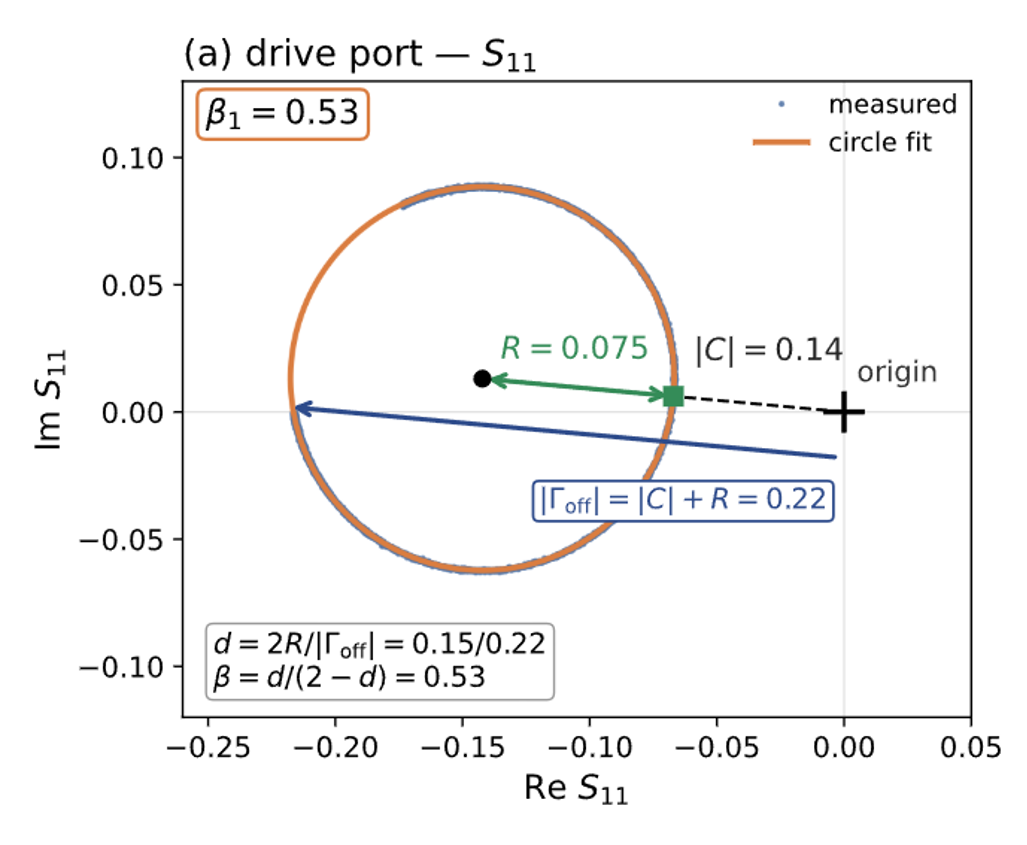
\includegraphics[width=\textwidth]{qcircle_s11.png}
        \caption{Drive port, $S_{11}$}
    \end{subfigure}
    \hfill
    \begin{subfigure}[b]{0.32\textwidth}
        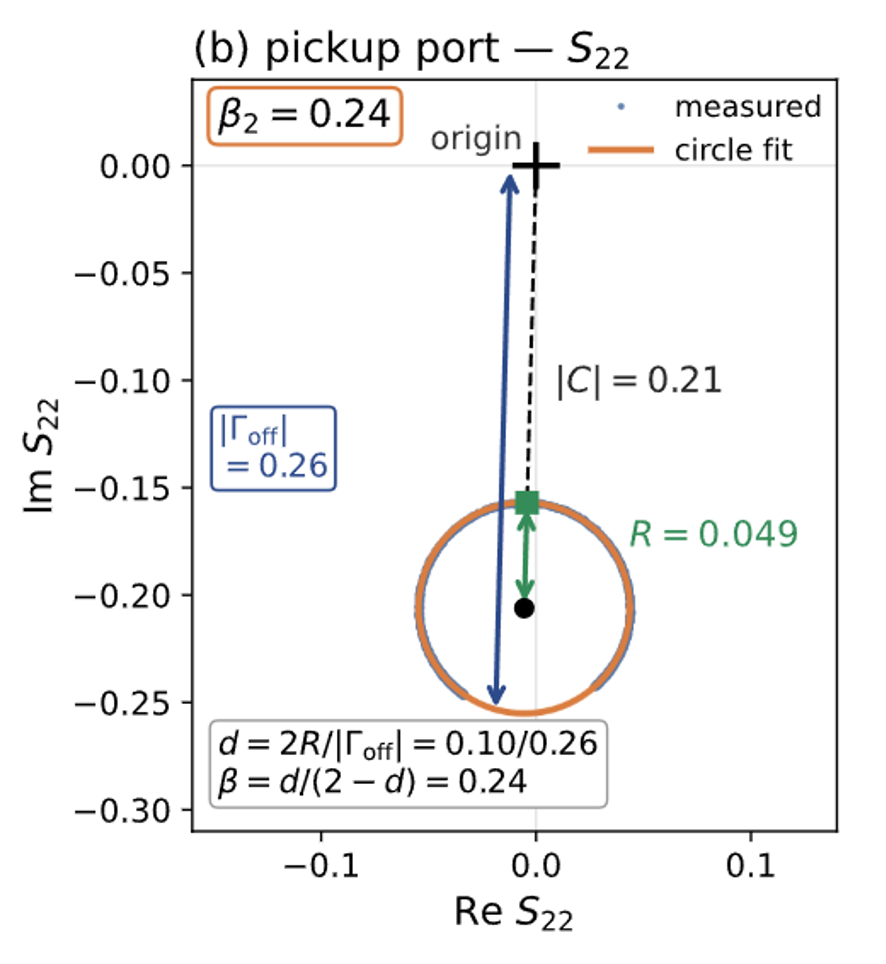
\includegraphics[width=\textwidth]{qcircle_s22.png}
        \caption{Pickup port, $S_{22}$}
    \end{subfigure}
    \hfill
    \begin{subfigure}[b]{0.32\textwidth}
        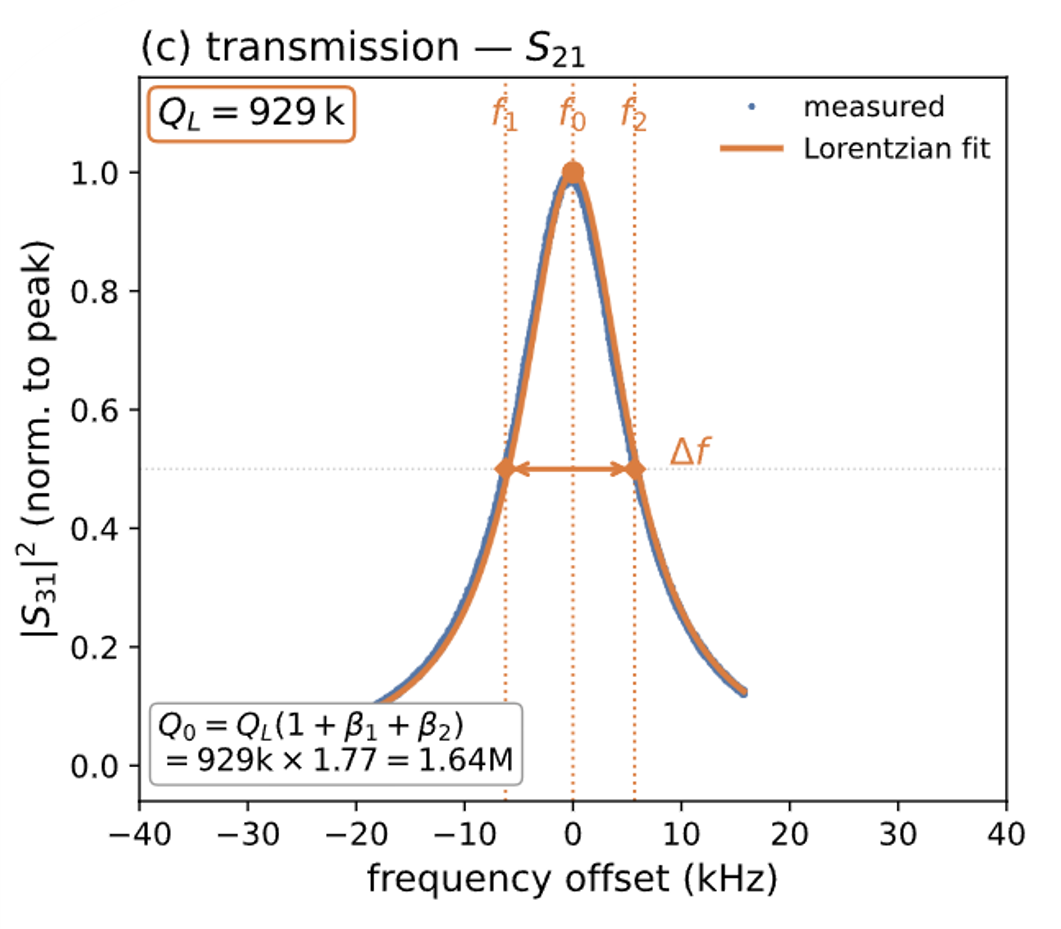
\includegraphics[width=\textwidth]{qcircle_s21.png}
        \caption{Transmission, $S_{21}$}
    \end{subfigure}
    \caption{Diameter-correction circle fits to the \SI{2}{\kelvin} drive-port (a) and pickup-port (b) reflection data, giving $\beta_1=0.53$ and $\beta_2=0.24$, and the Lorentzian fit to transmission (c) giving $Q_L=929{,}000$. Eq.~\eqref{eq:q0} combines these into $Q_0 = 1.64\times10^{6}$.}
    \label{fig:qcircle}
\end{figure*}

\section{Electromagnetic Simulation}

% --- Ported/adapted from repo app_q_correction.tex "Surface-specific
% geometric factors" section -- your own general G_i/COMSOL procedure. ---
The geometric factor of the cavity mode is
\begin{equation}
G = \frac{\int_V |\mu \vec{H}|^2\, dV}{\int_{S} |\vec{H}_\text{tan}|^2\, dS},
\label{eq:G_definition}
\end{equation}
with the stored magnetic energy in the numerator and the tangential field integrated over the RF surface in the denominator. $G$ is computed numerically: model the geometry with perfectly conducting walls, solve for the mode of interest (TM$_{010}$), extract the magnetic energy $U_m$, integrate the tangential field over the surface, and evaluate $G = 2U_m/I$.

\TODO{Mode-identification paragraph: TM$_{010}$ at $f_0=11.030$ GHz, TM$_{011}$ at 11.395 GHz, TM$_{012}$ at 12.399 GHz (Fig.~\ref{fig:sim}) -- these specific frequencies are dataset facts from your simulation, port directly if correct, just needs a sentence of your own framing for why identifying neighboring modes mattered.}

Combined with a literature bulk-copper conductivity, the same simulation gives a simulated bare-copper ceiling. \TODO{main.tex reports $Q_0=77{,}000$ ($R_s=5.00\,\mathrm{m}\Omega$) here, but your own thesis/repo correction work (Eq.~8.3 in thesis, and app\_q\_correction.tex) uses $Q_\text{Cu,ideal}=76{,}000$ for the same $G=350\,\Omega$ seamless geometry -- 76k vs 77k, close but not identical. Check which is the correct current simulated value for this specific hexagonal cavity before finalizing.}

\begin{figure*}[!t]
    \centering
    
\includegraphics[width=0.85\textwidth]{sim_modes.png}
    \caption{Simulated electric field norm for the fundamental TM$_{010}$ mode and the two nearest higher-order modes, TM$_{011}$ and TM$_{012}$, used to confirm mode identity and to extract the geometric factor $G=\SI{350}{\ohm}$.}
    \label{fig:sim}
\end{figure*}

\section{Results and Discussion}

\TODO{Main results paragraph -- no direct thesis passage exists for the Ta/Nb dataset. Your thesis DOES use the identical correction-factor logic pattern for the Nb3Sn cavity (Ch.~8, ``Correction 2: Accounting for RF Leakage''): $\alpha = Q_{\text{Cu,ideal}}/Q_{\text{Cu,measured}}$, there evaluated as $76{,}000/55{,}000=1.38$. You could reuse that sentence structure here, adapted to the Ta/Nb numbers -- but note main.tex uses UPDATED poster numbers (measured Cu $Q_0=62{,}000$, simulated Cu $Q_0=77{,}000$) rather than your thesis's older Nb3Sn-era Cu numbers (55,000 / 76,000). Facts to weave in, in your own words:
\begin{itemize}
\item Film at 2 K: $Q_0=1.64\times10^6$, $R_s=213\,\mu\Omega$.
\item vs. measured bare-Cu baseline ($Q_0=62{,}000$, $R_s=5.65\,\mathrm{m}\Omega$): $\sim$26$\times$ improvement.
\item Consistent with simulated bulk-Cu ceiling ($Q_0=77{,}000$) -- confirms the Cu baseline is representative, not an outlier.
\item Separate finding: sealing the bare-Cu cavity's seam with indium foil raised $Q_0$ from 55,000 to 62,000 -- a lead for future work, not yet applied to the coated cavity.
\item vs. BCS-limited Nb at 2 K ($R_s\approx0.58\,\mu\Omega$, $Q_0\approx6.0\times10^8$): measured film $\sim$250$\times$ higher in $R_s$.
\end{itemize}}

\begin{figure*}[!t]
    \centering
    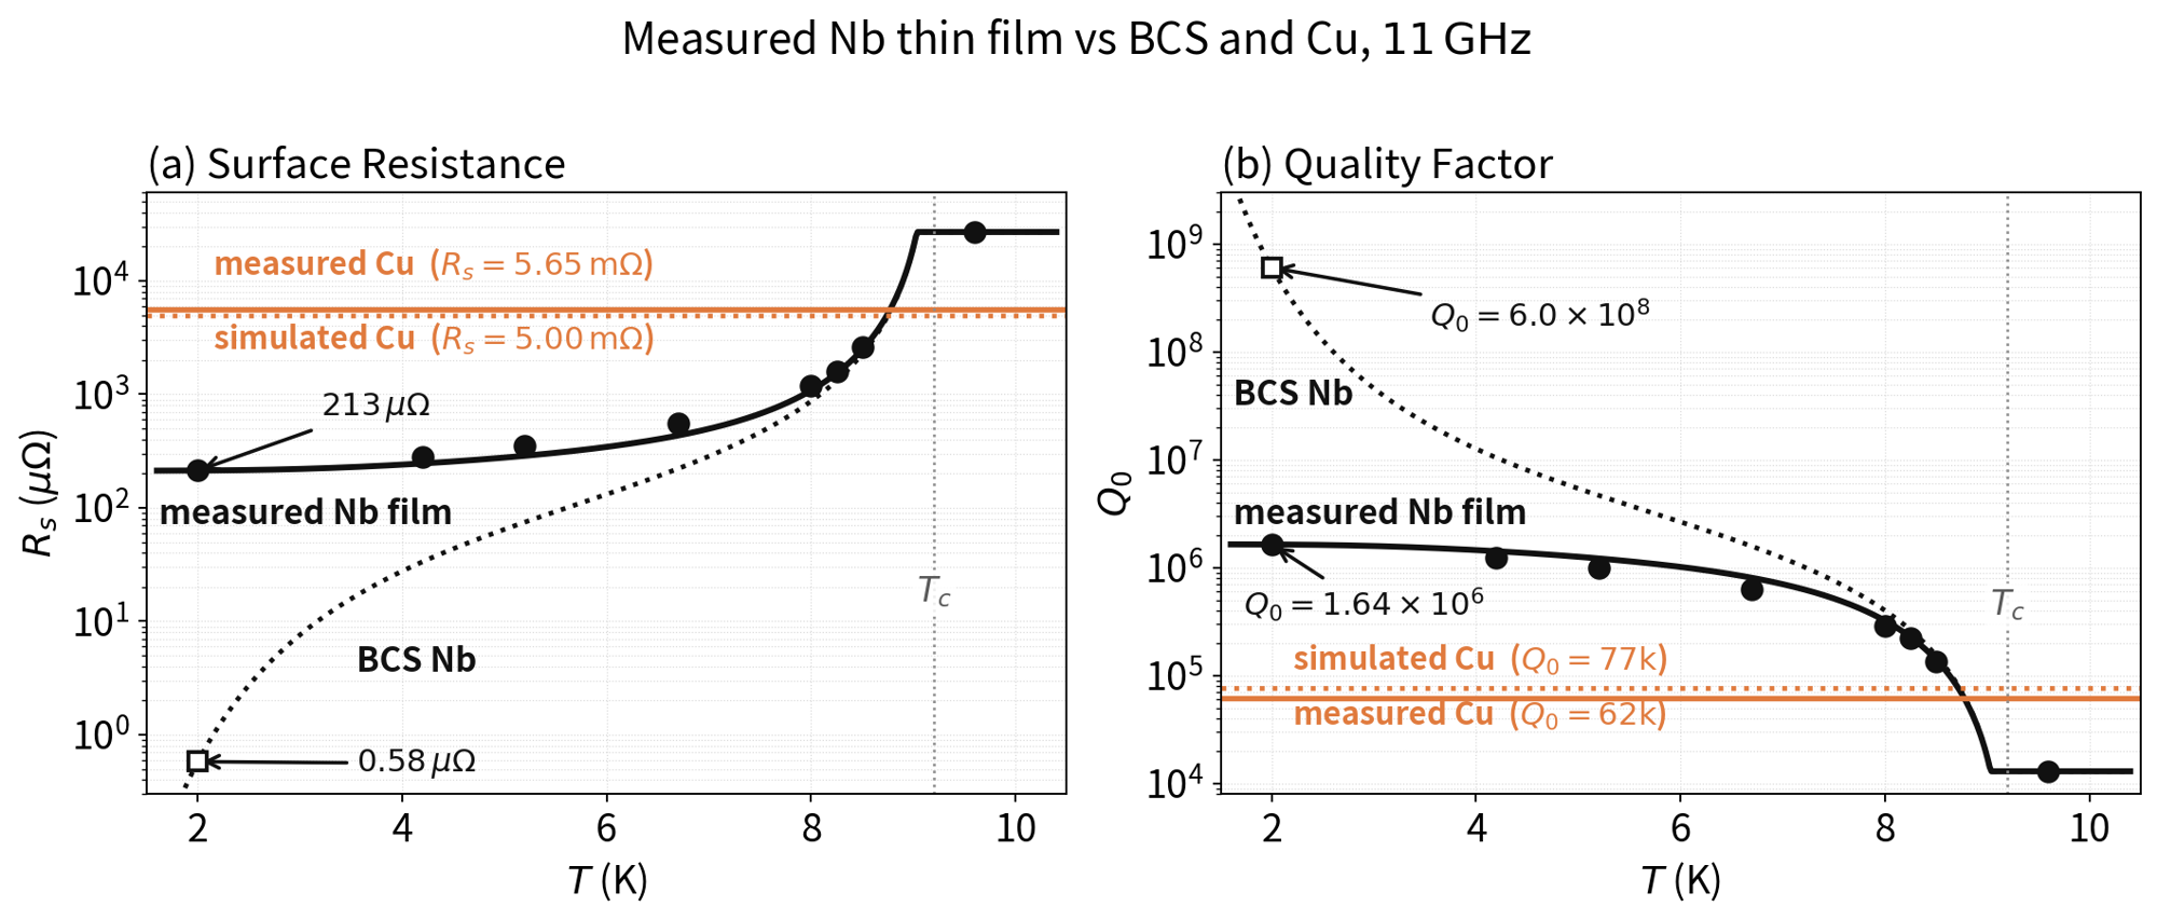
\includegraphics[width=0.85\textwidth]{rs_q0_vs_T.png}
    \caption{Measured surface resistance (a) and unloaded quality factor (b) of the Ta/Nb-coated cavity versus temperature at 11\,GHz and zero field, compared against BCS Nb, the measured bare-Cu baseline, and the simulated bulk-Cu ceiling.}
    \label{fig:results}
\end{figure*}

\TODO{Roughness/flux-trapping discussion -- entirely new argument from this session, no prior draft exists. Logic: the 250$\times$ BCS gap is too large to attribute to trapped-flux resistance (small at realistic ambient fields); surface roughness enhancing local current path length/field at grain boundaries is the more likely dominant term. Fig.~\ref{fig:roughness} (Veeco confocal scan) shows $\pm2\,\mu$m background roughness with grooves to $-8$ to $-11\,\mu$m. For comparison, electropolished Nb-on-Cu films in the literature reach AFM roughness (Ra) of only 6--21 nm~\cite{Pira2019CuPolish} -- two to three orders of magnitude below what you measured. Write this argument in your own words; the citation and the scan data are solid, the interpretation prose is mine.}

\begin{figure}[!t]
    \centering
    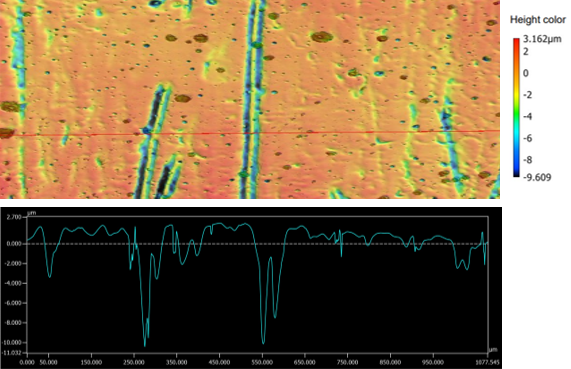
\includegraphics[width=0.95\linewidth]{roughness.png}
    \caption{Laser-scanning confocal microscope (Veeco) height map of the sputtered Nb surface (top; red line marks the scan location) and the corresponding line-scan height profile (bottom), showing $\pm$\SI{2}{\micro\meter} background roughness with scattered grooves reaching \SIrange{-8}{-11}{\micro\meter}.}
    \label{fig:roughness}
\end{figure}

% --- Adapted from thesis diffusion-barrier discussion ("Ta and Nb both
% effective at blocking Cu interdiffusion") -- your own reasoning pattern for
% why a clean transition confirms barrier performance, applied here to Tc. ---
Approaching the transition, $R_s$ rises gradually before increasing sharply near \SI{9.2}{\kelvin}, matching the bulk-Nb critical temperature. Above $T_c$, $Q_0$ falls to order $10^{4}$, below the bare-copper baseline, because normal-state Nb is more resistive than annealed copper and the film exceeds its normal-state skin depth at \SI{11}{\giga\hertz}. That the transition sits at the bulk-Nb $T_c$, rather than at a suppressed value indicative of Cu interdiffusion, confirms that the Ta layer is an effective diffusion barrier and that the sputtered film is close to stoichiometric bulk Nb. \TODO{Adapt wording -- your existing barrier-comparison table (thesis) discusses Ta/Nb/W barriers for Nb3Sn diffusion specifically; this is the same underlying logic (clean transition = effective barrier) applied to your Ta/Nb control cavity instead.}

\section{Conclusion}

\TODO{Model tone/structure on your own thesis Sec.~9.1 conclusion (numbered-results style), but content is new since the thesis has no Ta/Nb-only chapter. Should recap: $Q_0=1.64\times10^6$ at 2 K, $\sim$26$\times$ over Cu, $\sim$250$\times$ above BCS-Nb (roughness-dominated), clean $T_c$ transition confirms barrier, PPMS-compact-platform framing, and future work (indium seal on coated cavity, roughness characterization, HiPIMS Nb, Nb3Sn by Cu-Sn route).}

\section*{Acknowledgment}
This work is supported by the U.S. Department of Energy, Office of Science, Office of High Energy Physics and the Accelerator R\&D and Production (ARDAP) office, under Award No.\ DE-SC0018379 and DE-SC0026206. A portion of this work was performed at the National High Magnetic Field Laboratory, which is supported by the National Science Foundation Cooperative Agreement No.\ DMR-1644779 and the State of Florida.

\begin{thebibliography}{9}

\bibitem{ADMX:2009iij}
S.~J.~Asztalos \emph{et al.}, ``SQUID-based microwave cavity search for dark-matter axions,'' \emph{Phys. Rev. Lett.}, vol.~104, no.~4, p.~041301, 2010.

\bibitem{Braine:2024nzi}
T.~Braine, ``Superconducting resonator development for the Axion Dark Matter eXperiment,'' arXiv:2408.03444 [hep-ex], 2024.

\bibitem{Ciovati:2014zti}
G.~Ciovati, ``AC/RF superconductivity,'' arXiv:1501.07398 [physics.acc-ph], 2014.

\bibitem{gurevichUseNotUse2011}
A.~Gurevich, ``To use or not to use cool superconductors?,'' \emph{Nature Mater.}, vol.~10, no.~4, pp.~255--259, 2011.

\bibitem{posenNb3SnSuperconductingRadiofrequency2017}
S.~Posen and D.~L.~Hall, ``Nb$_3$Sn superconducting radiofrequency cavities: fabrication, results, properties, and prospects,'' \emph{Supercond. Sci. Technol.}, vol.~30, no.~3, p.~033004, 2017.

\bibitem{withanageRapidNbSn2021}
W.~Withanage, A.~Juliao, and L.~Cooley, ``Rapid Nb$_3$Sn film growth by sputtering Nb on hot bronze,'' \emph{Supercond. Sci. Technol.}, vol.~34, 2021.

\bibitem{fonnesuRecipeOptimizationSRF2025}
D.~Fonnesu \emph{et al.}, ``Recipe optimization and SRF test of Cu-compatible Nb$_3$Sn films by DC magnetron sputtering from a stoichiometric target,'' Research Square preprint, 2025.

\bibitem{sayeedFabricationSuperconductingNb3Sn2023}
M.~N.~Sayeed, U.~Pudasaini, G.~V.~Eremeev, and H.~E.~Elsayed-Ali, ``Fabrication of superconducting Nb$_3$Sn film by co-sputtering,'' \emph{Vacuum}, vol.~212, p.~112019, 2023.

\bibitem{posen2023HighQ}
S.~Posen \emph{et al.}, ``High-quality-factor superconducting cavities in Tesla-scale magnetic fields for dark-matter searches,'' \emph{Phys. Rev. Appl.}, vol.~20, p.~034004, 2023.

\bibitem{alesini2019QUAX}
D.~Alesini \emph{et al.}, ``Galactic axions search with a superconducting resonant cavity,'' \emph{Phys. Rev. D}, vol.~99, p.~101101, 2019.

\bibitem{oikawaMushroomCavity2019}
Y.~Oikawa \emph{et al.}, ``Fabrication of Nb mushroom shaped cavity for evaluation of multi-layer thin-film superconductor,'' in \emph{Proc. 29th Linear Accelerator Conf. (LINAC2018)}, 2019, paper TUPO053.

\bibitem{luCuBronzeQPR2026}
M.~Lu \emph{et al.}, ``Preparation of the Cu-based Nb$_3$Sn sample via bronze route for quadrupole resonator testing,'' \emph{Supercond. Sci. Technol.}, 2026, doi: 10.1088/1361-6668/ae496a.

\bibitem{sealChokeCavity2025}
D.~Seal, ``Development of a high throughput facility for the RF characterisation of superconducting thin films,'' Ph.D. dissertation, Lancaster Univ., Dec. 2025.

\bibitem{KajfezHwan1984}
D.~Kajfez and E.~J.~Hwan, ``Q-factor measurement with network analyzer,'' \emph{IEEE Trans. Microw. Theory Tech.}, vol.~MTT-32, no.~7, pp.~666--670, Jul. 1984.

\bibitem{Pira2019CuPolish}
C.~Pira \emph{et al.}, ``Impact of the Cu substrate surface preparation on the morphological, superconductive and RF properties of the Nb superconductive coatings,'' in \emph{Proc. 19th Int. Conf. RF Superconductivity (SRF2019)}, Dresden, Germany, 2019, pp.~935--940.

\end{thebibliography}

\end{document}
